%! TEX root = ../../DesignDocument.tex
\hspace{7mm}
Before development on visual components of the project ensues, prototypes are mocked in a
design editor and approved by the development team.  The prototypes serve
as dynamic style guides moving forward with development and not a set-in-stone template
to steer development.\\

The following prototypes were created for web pages early in the development cycle.

\subsection{Website Home Page}
    \hspace{7mm} The style guide for the root login page of the ASP.NET website.
    From this page, users are able to log in to their account and navigate 
    one of three paths.
        \begin{itemize} 
            \item Upload a Model -
                A form where a user can browse their computer for 3D modol files to
                upload to the ASP.NET website under their account with a unique name. 
            \item My Models - 
                An environment where users can view, rename, download, or remove
                3D model files that they have previously uploaded to the website
            \item My Organization -
                An environment where users can join an existing organization account
                or view files and activity from other users who are active within 
                the same organization.
        \end{itemize}
    \ \\
    \label{fig:proto_web_home}
    \begin{figure}[H]
        \centering 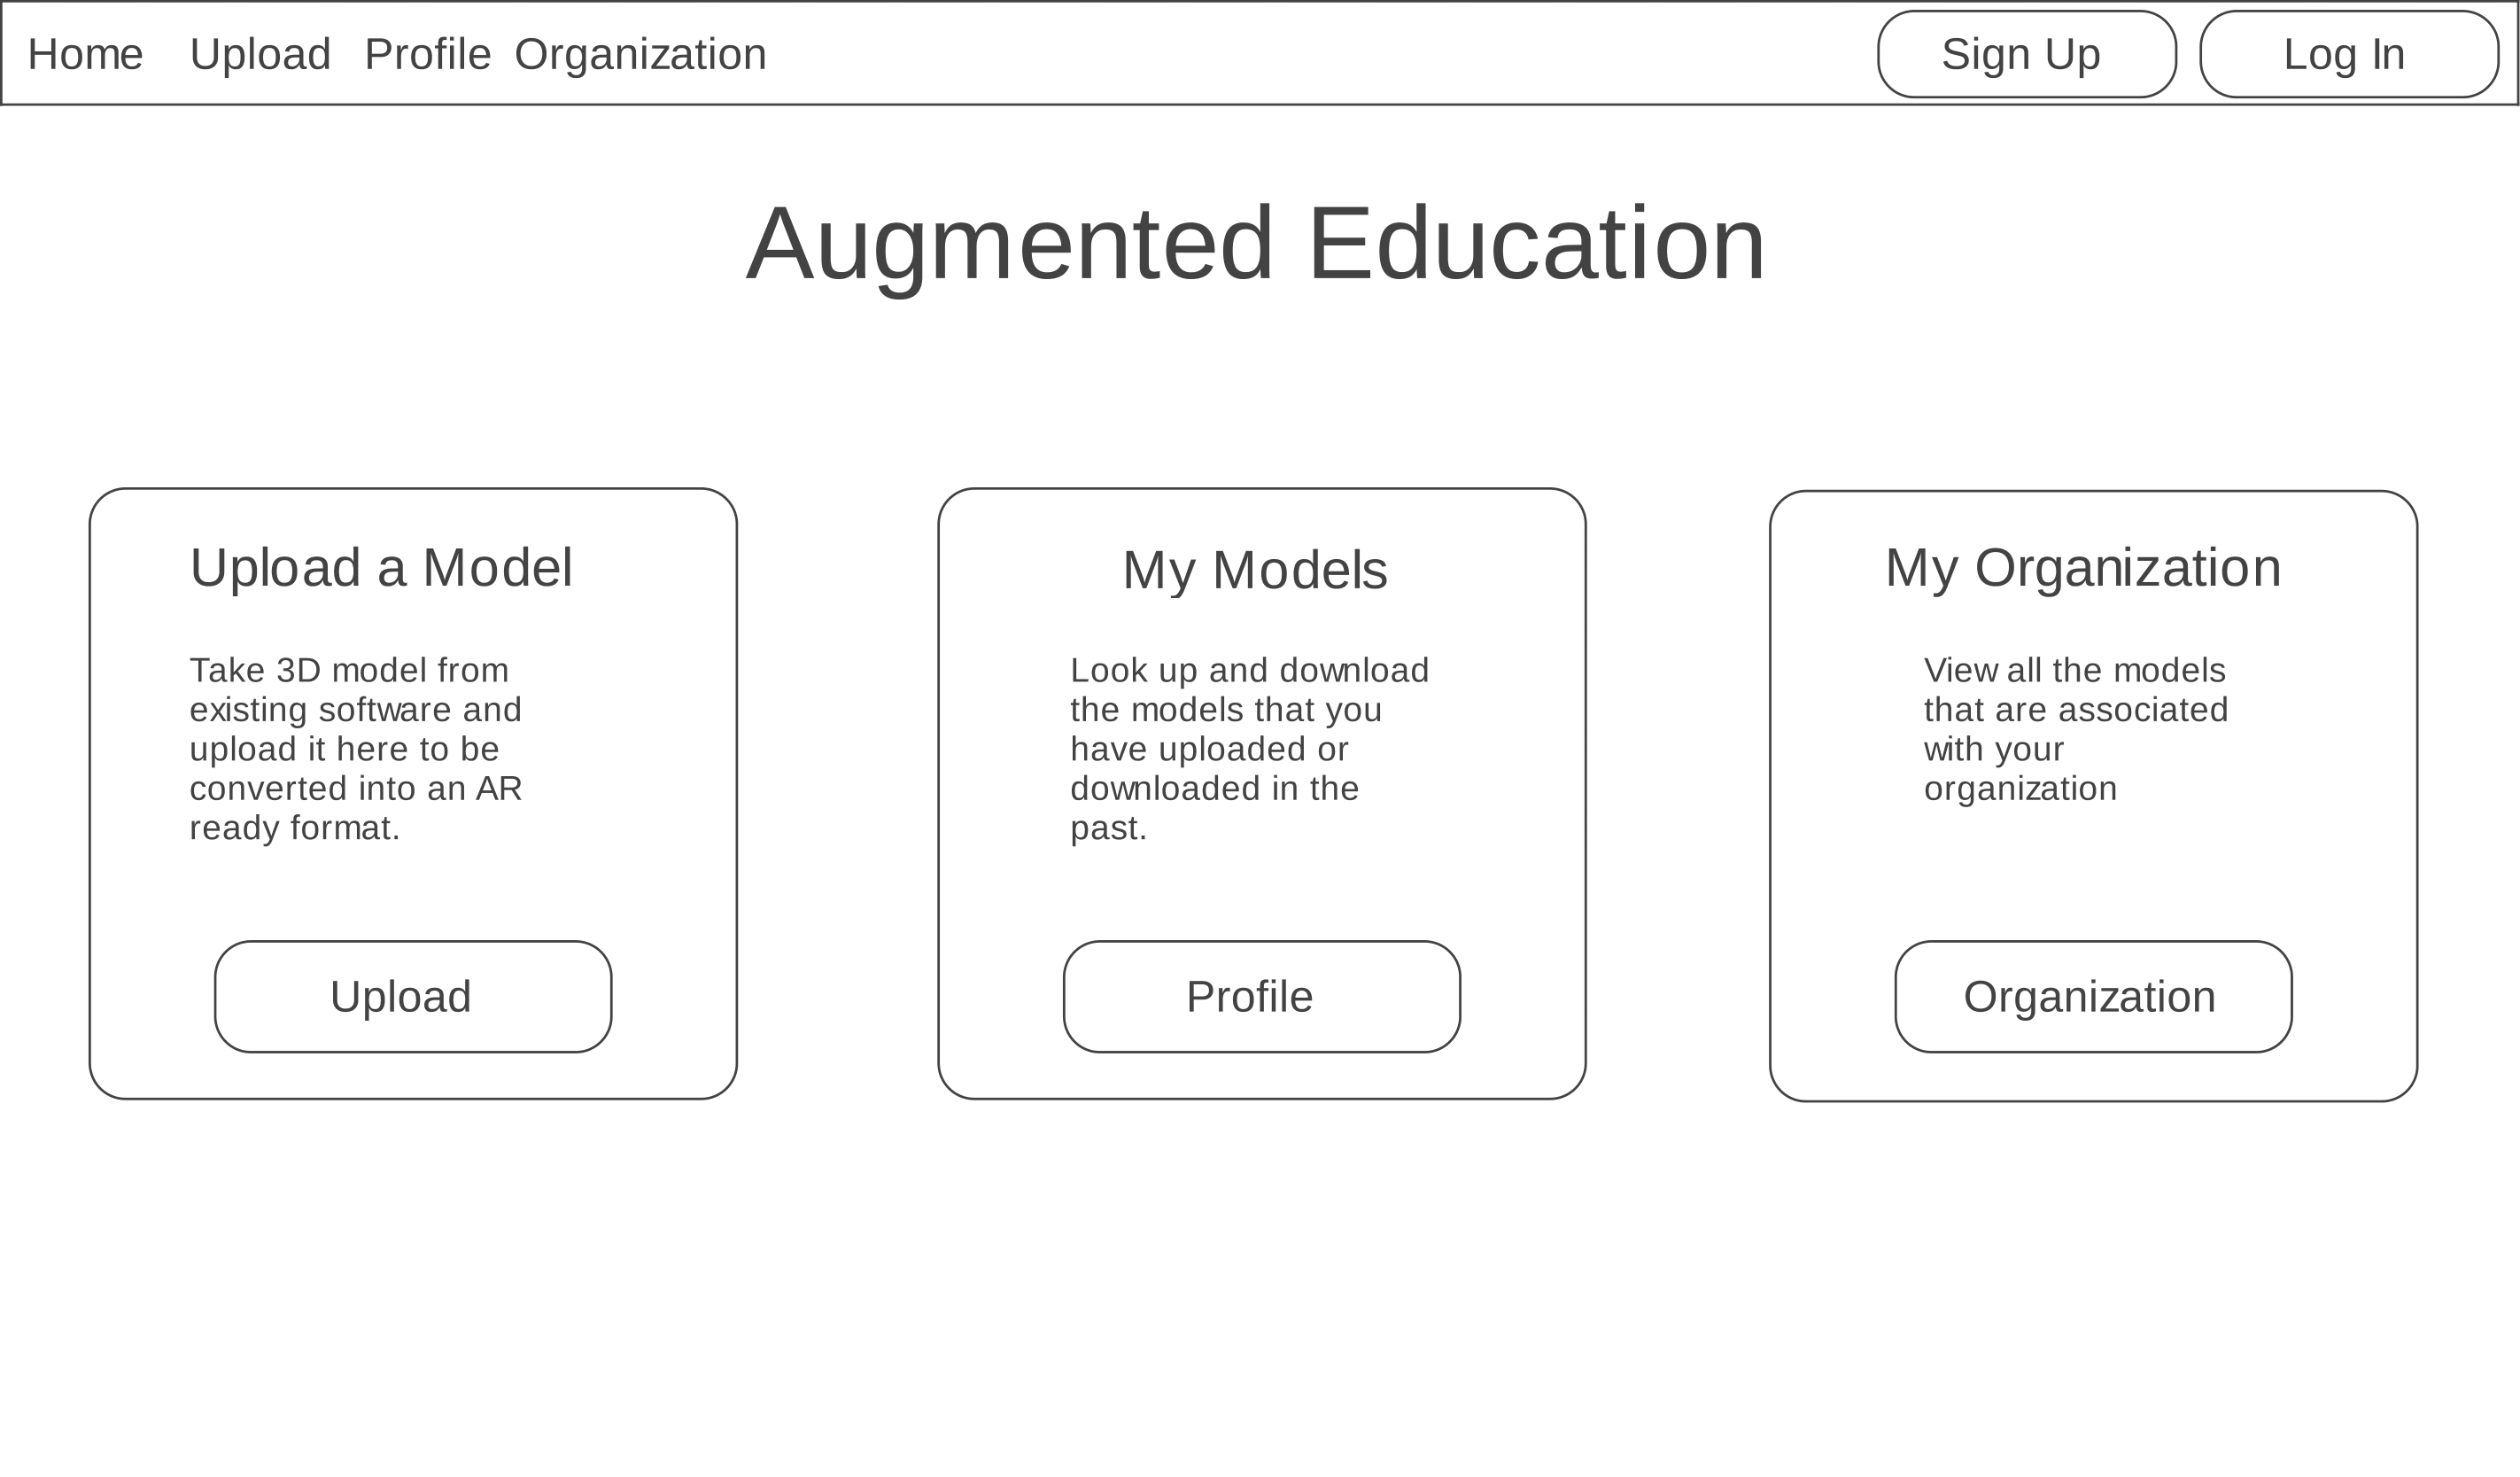
\includegraphics[width=0.6\linewidth]{Home}
        \caption{The wireframe for the website homepage}
    \end{figure}

\newpage
\subsection{File Upload Page}
    \hspace{7mm} The style guide for the page where a user can fill out a form 
    that allows them to browse to a 3D model file on their computer and upload
    it to the ASP.NET website under their user account.
    \ \\
    \label{fig:proto_web_upload}
    \begin{figure}[H]
        \centering 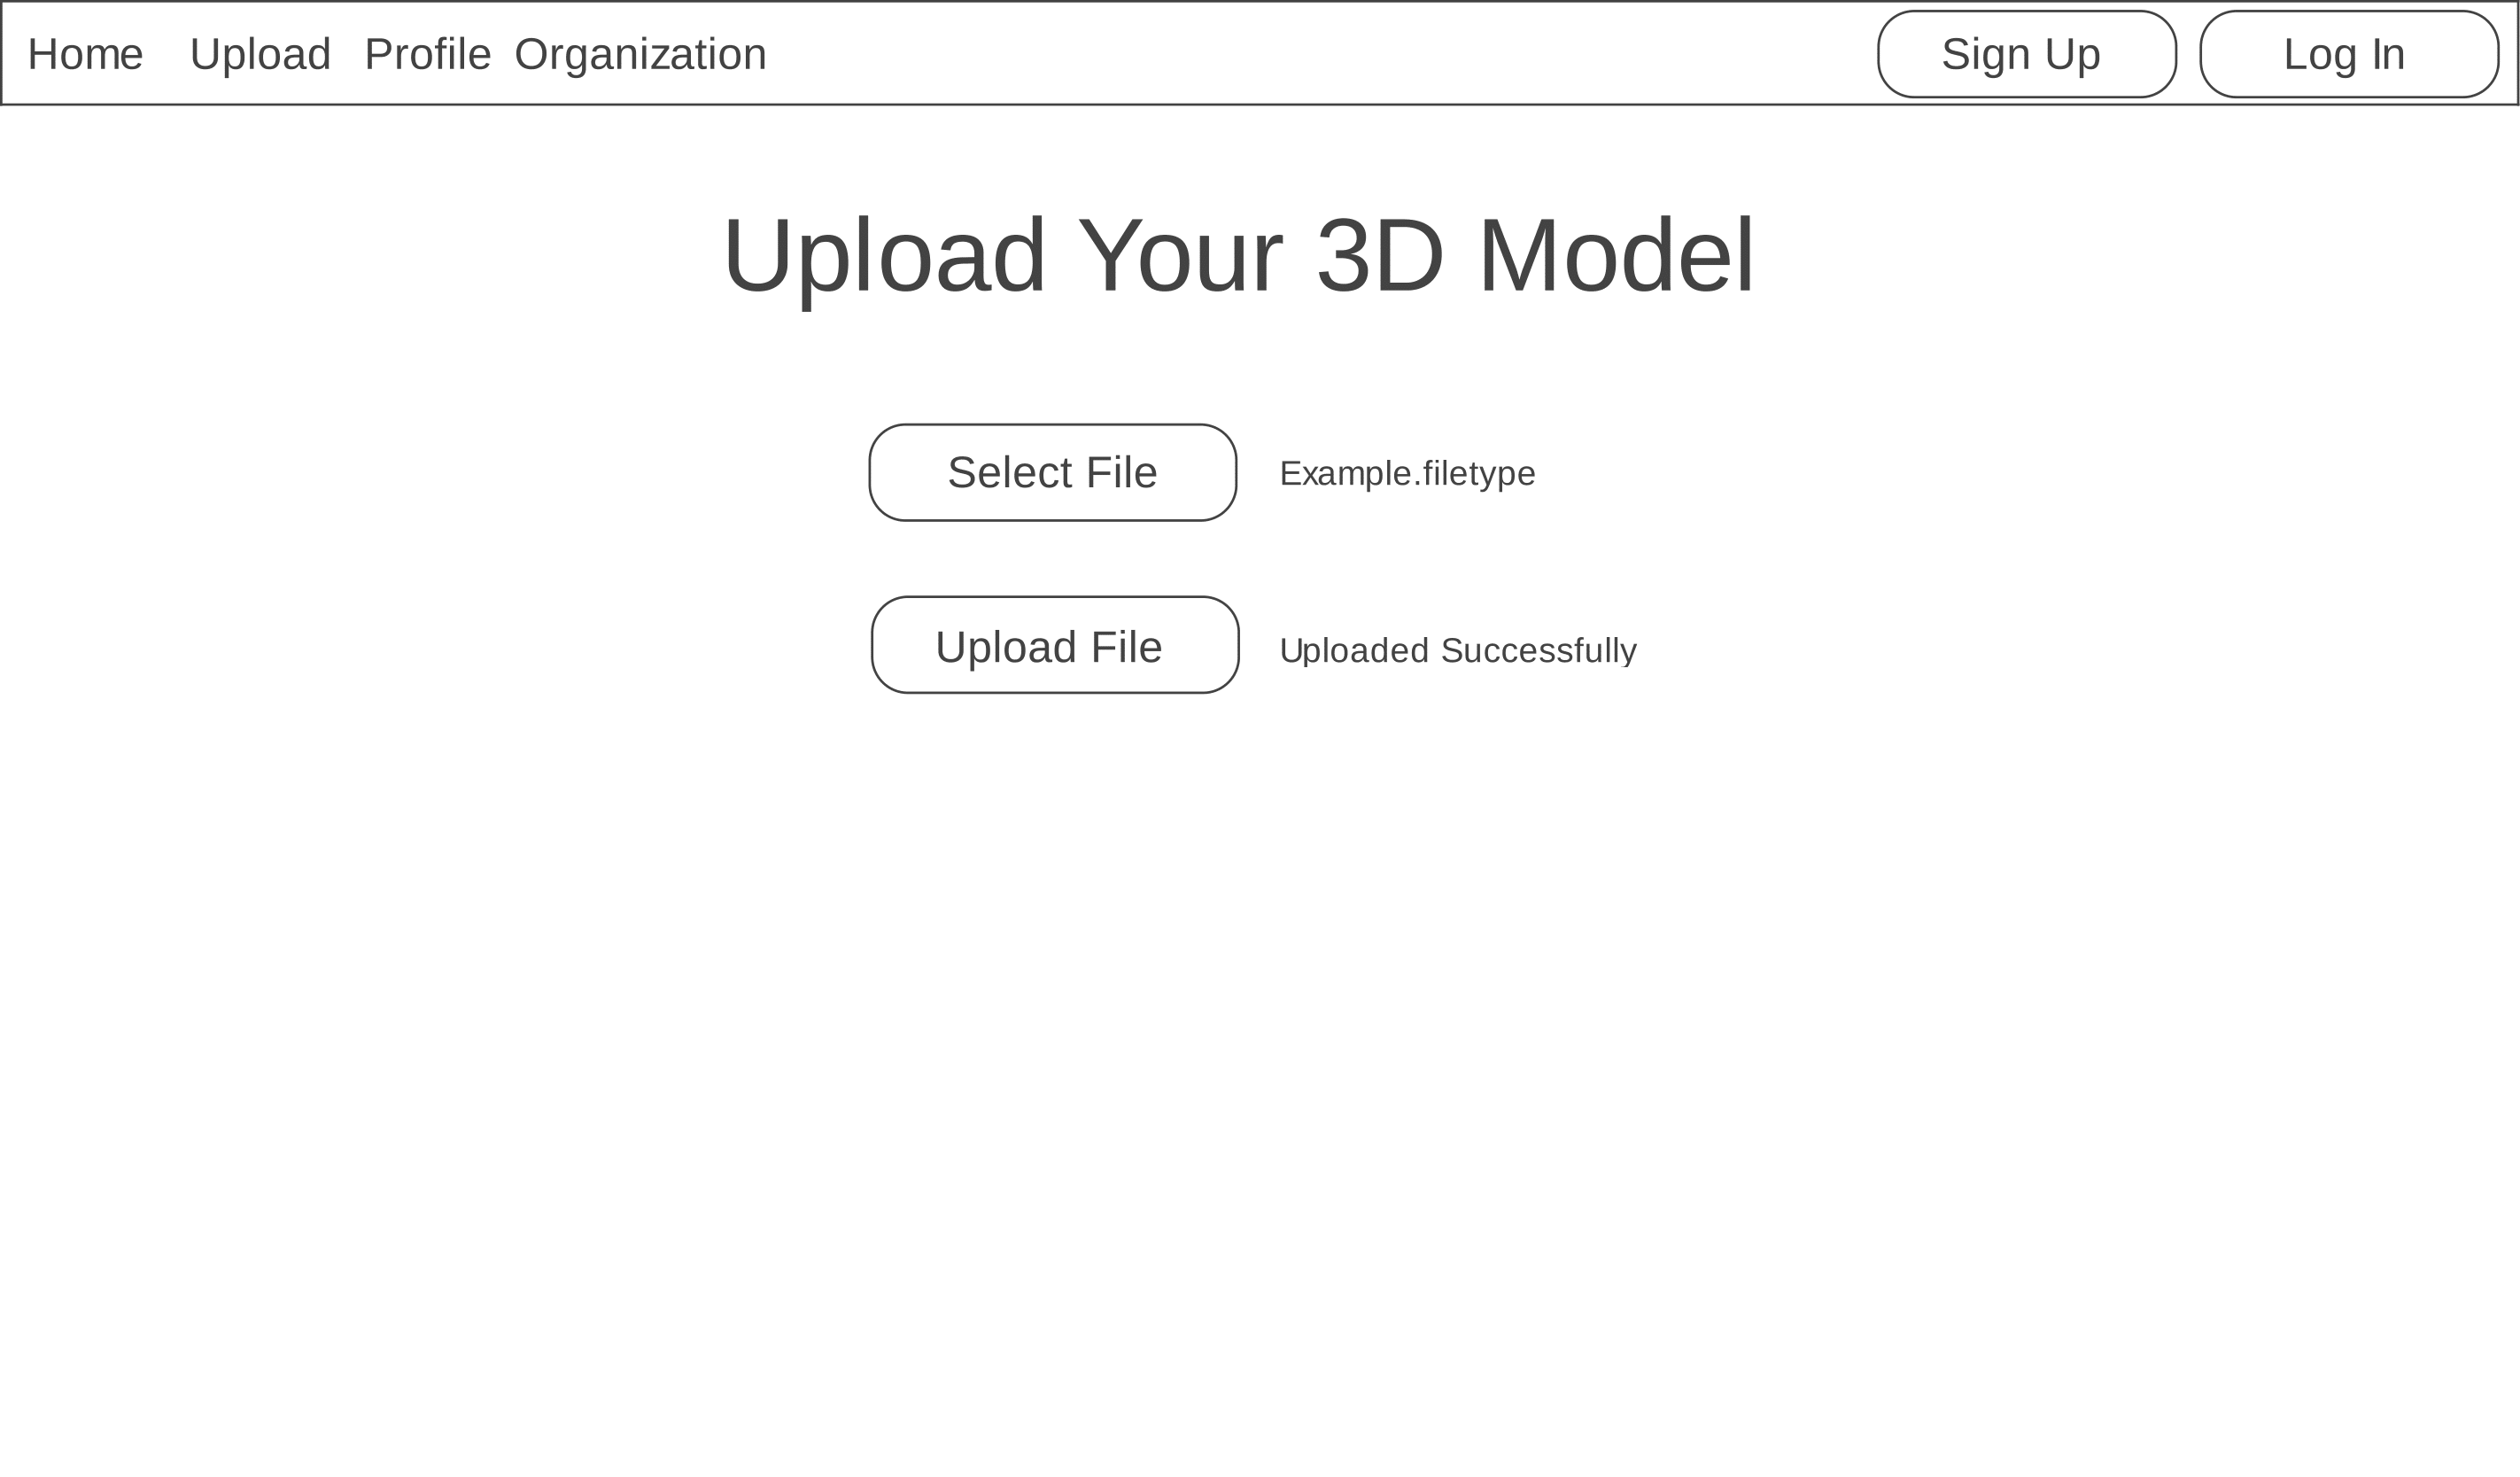
\includegraphics[width=0.6\linewidth]{Upload}
        \caption{The wireframe for the upload page form}
    \end{figure}

\subsection{User specific page}
    \hspace{7mm}
    An environment where a user can view all of their uploaded files being stored 
    on the cloud as well as a recent activity log.
    \ \\
    \label{fig:proto_web_user_page}
    \begin{figure}[H]
        \centering 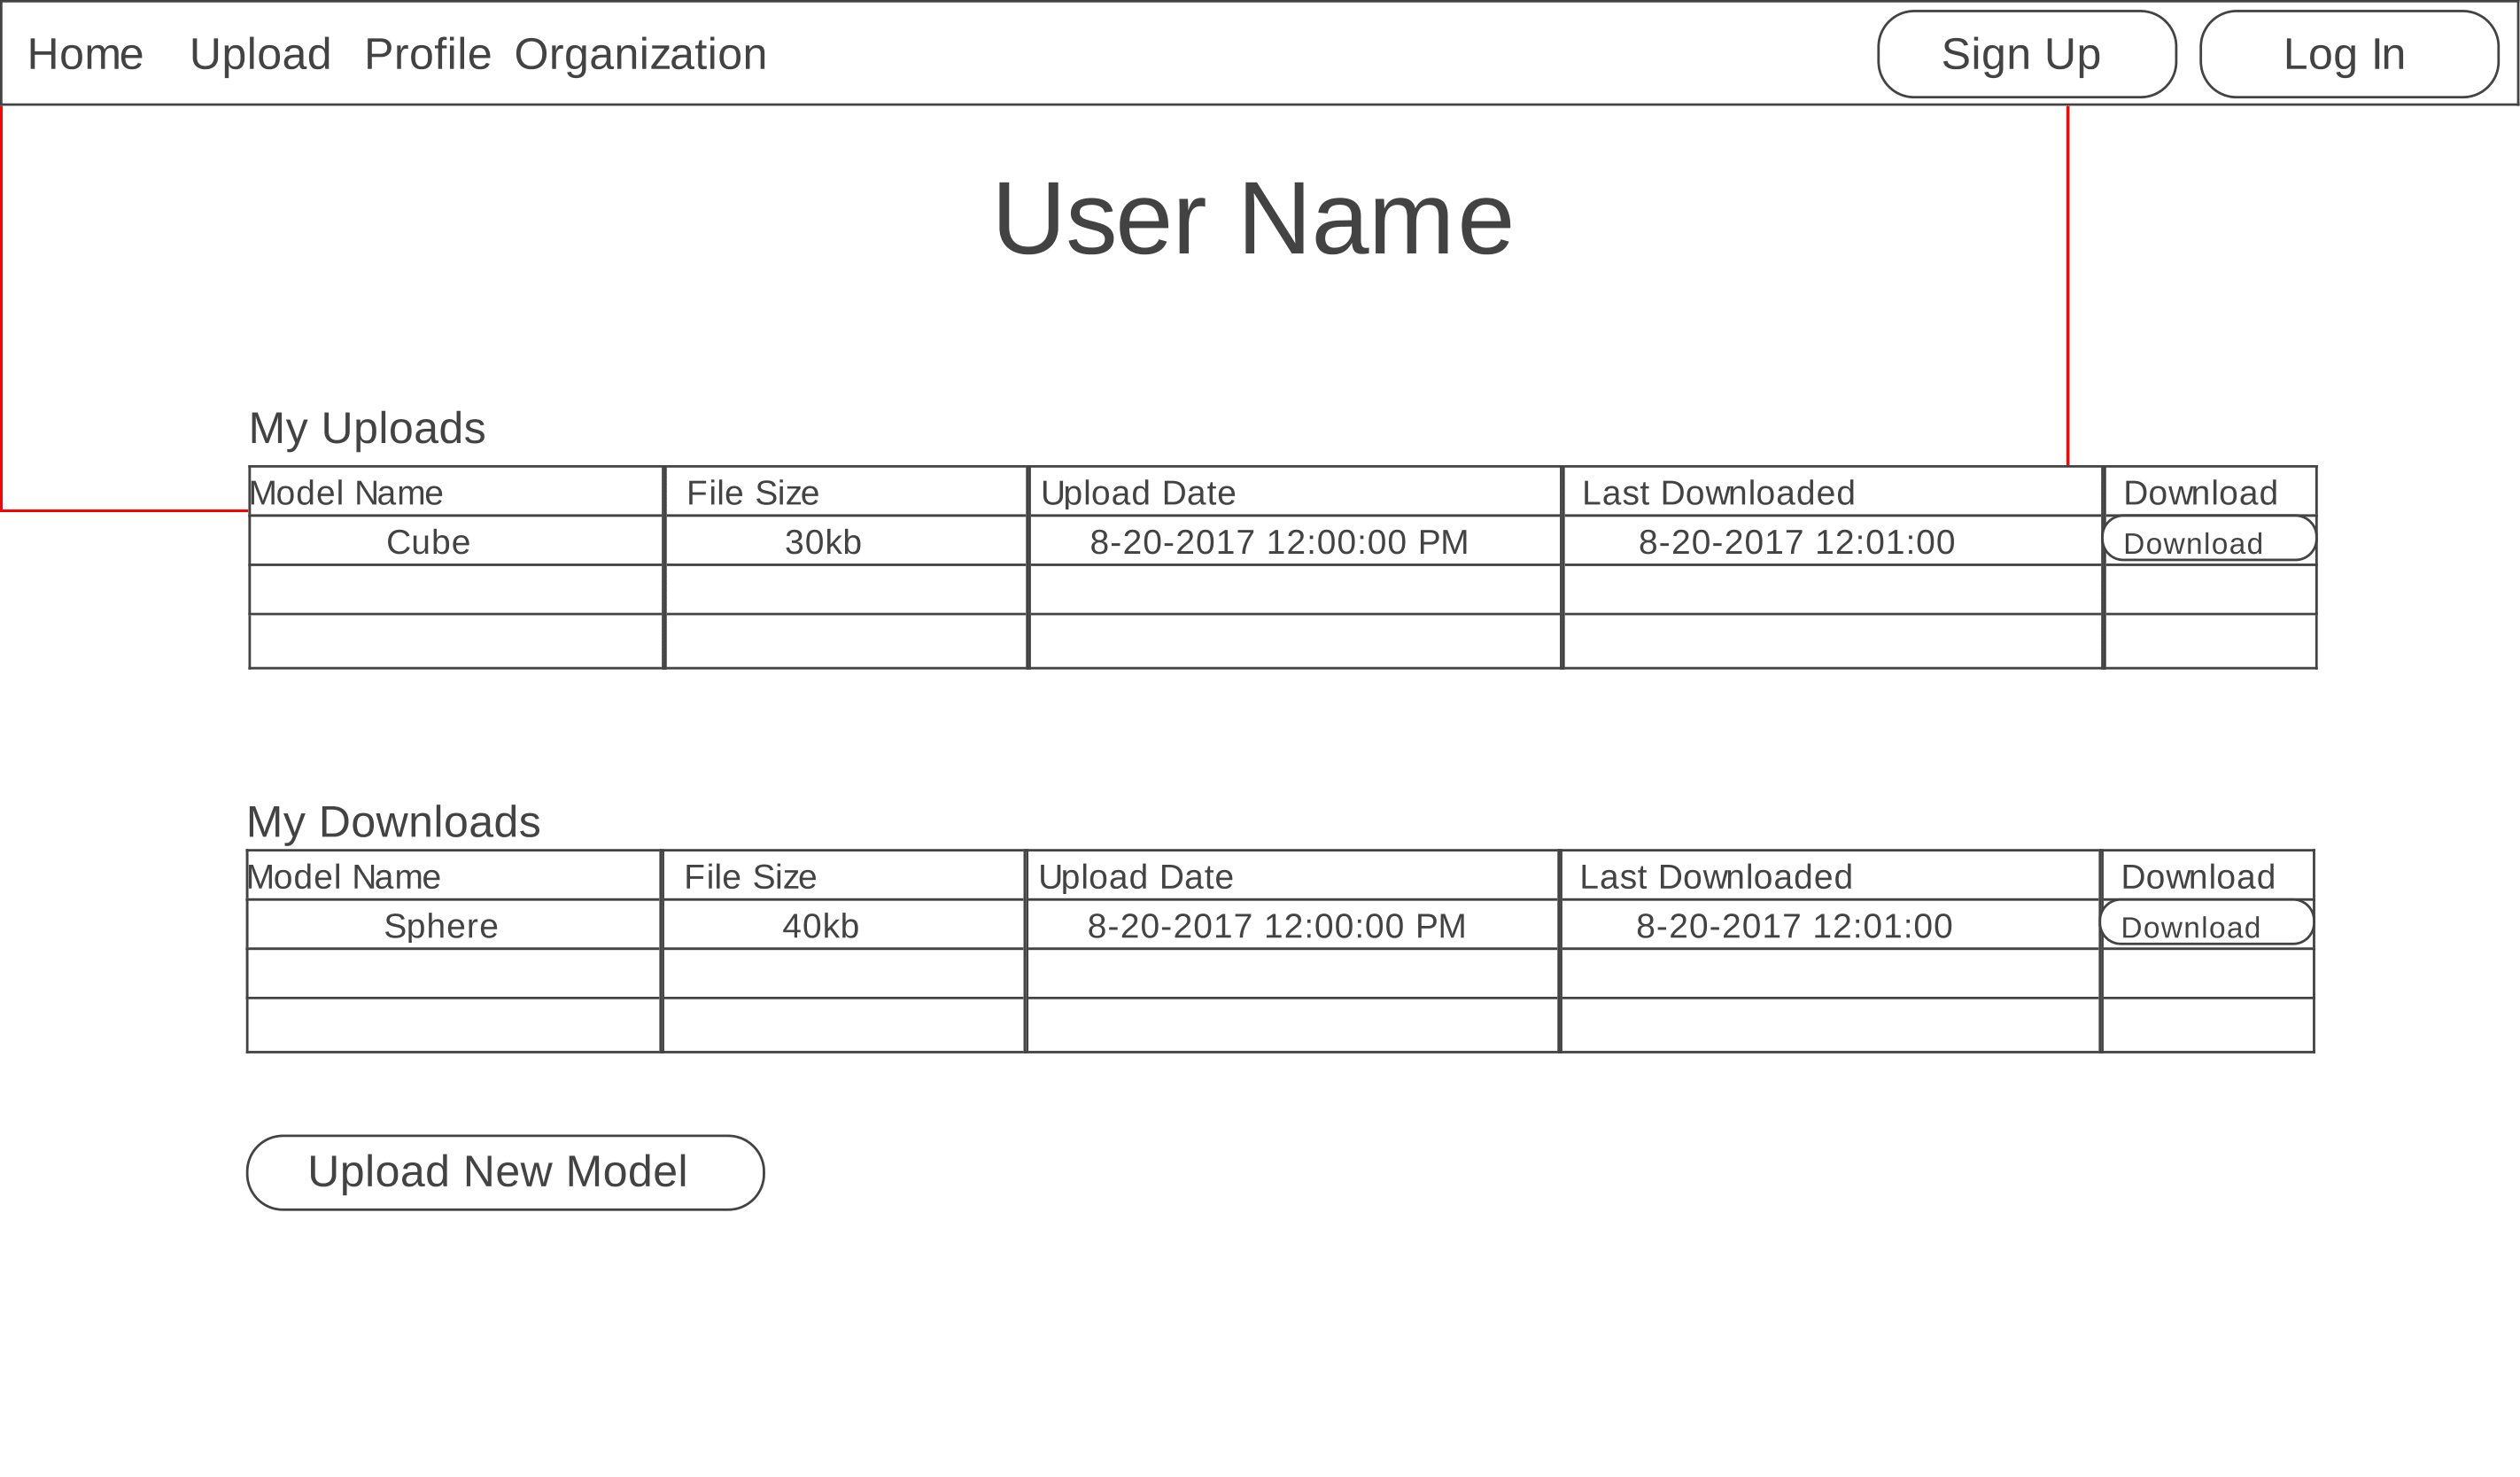
\includegraphics[width=0.6\linewidth]{UserPage}
        \caption{The wireframe for a user's account page}
    \end{figure}

\newpage
\subsection{The Organization home page}
    \hspace{7mm}
    The environment where users can view files and activity from other users who are
    active within the same organization.
    \ \\
    \label{fig:proto_web_organization_home}
    \begin{figure}[H]
        \centering 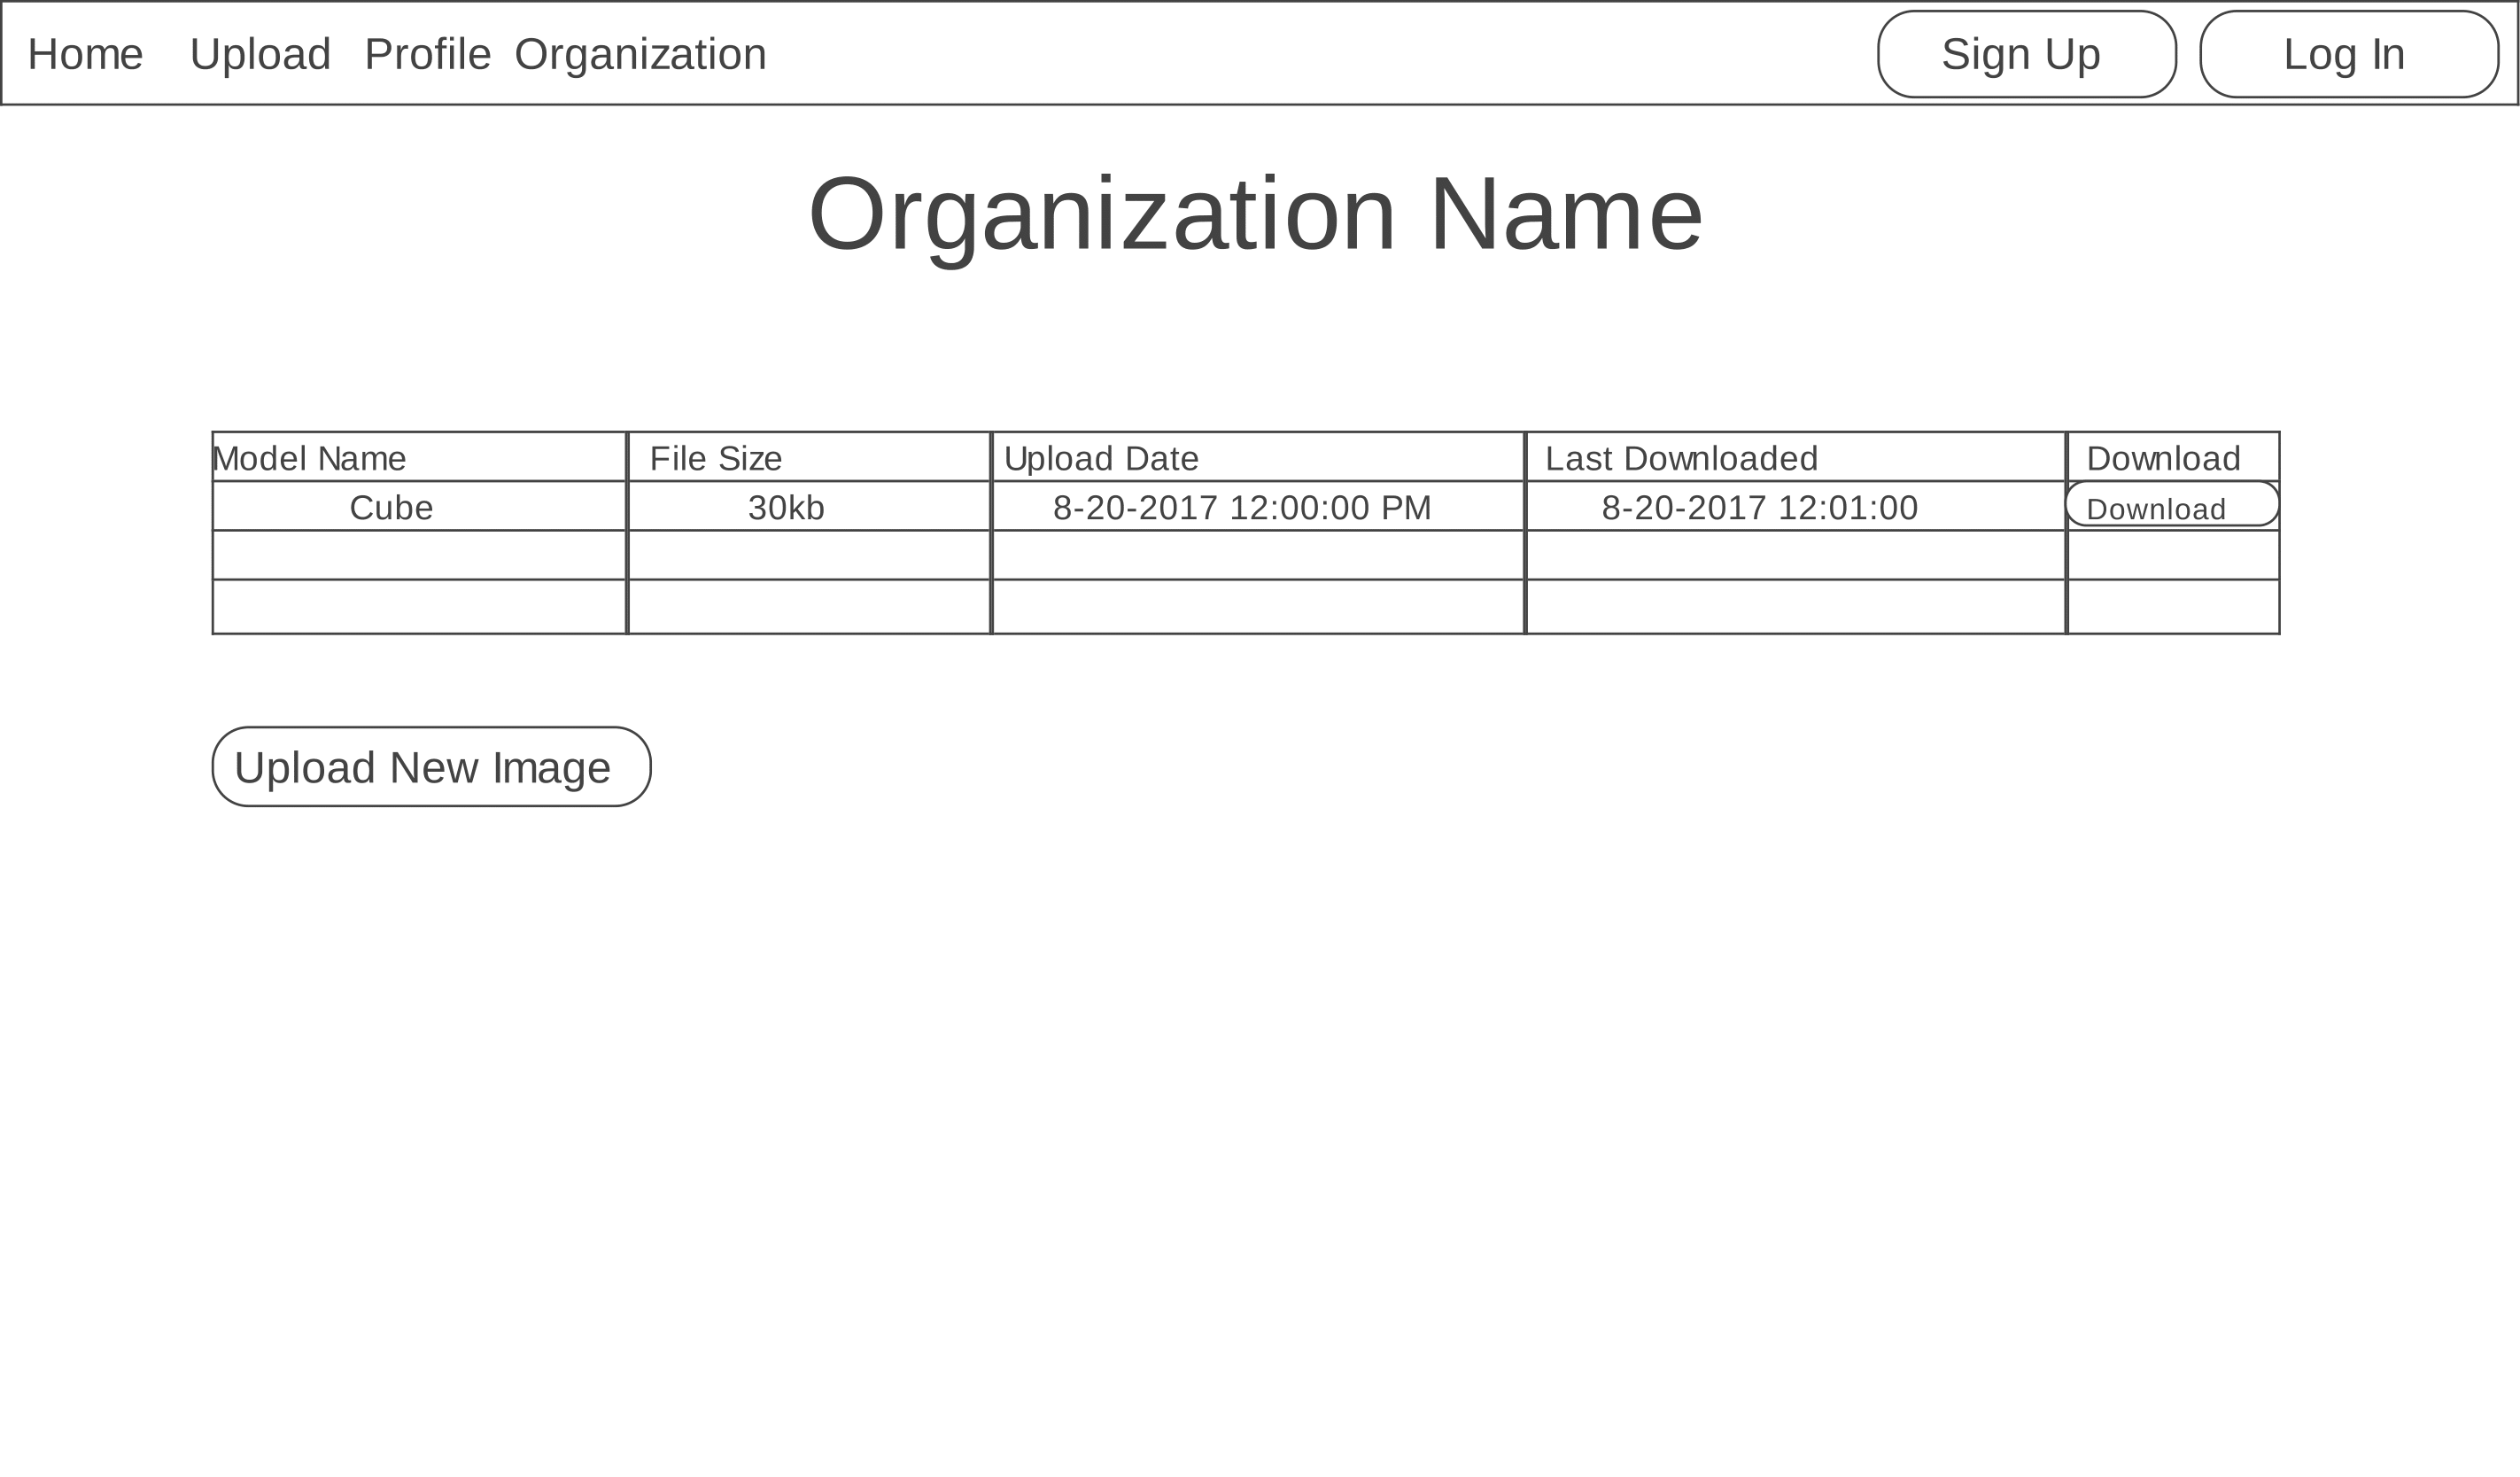
\includegraphics[width=0.6\linewidth]{Organization}
        \caption{The wireframe for an organization's home page}
    \end{figure}

\subsection{All available files}
    \hspace{7mm}
    An environment where users can view all files hosted on the cloud server that
    they have permission to view or download.
    \ \\
    \label{fig:proto_web_browse_all_files}
    \begin{figure}[H]
        \centering 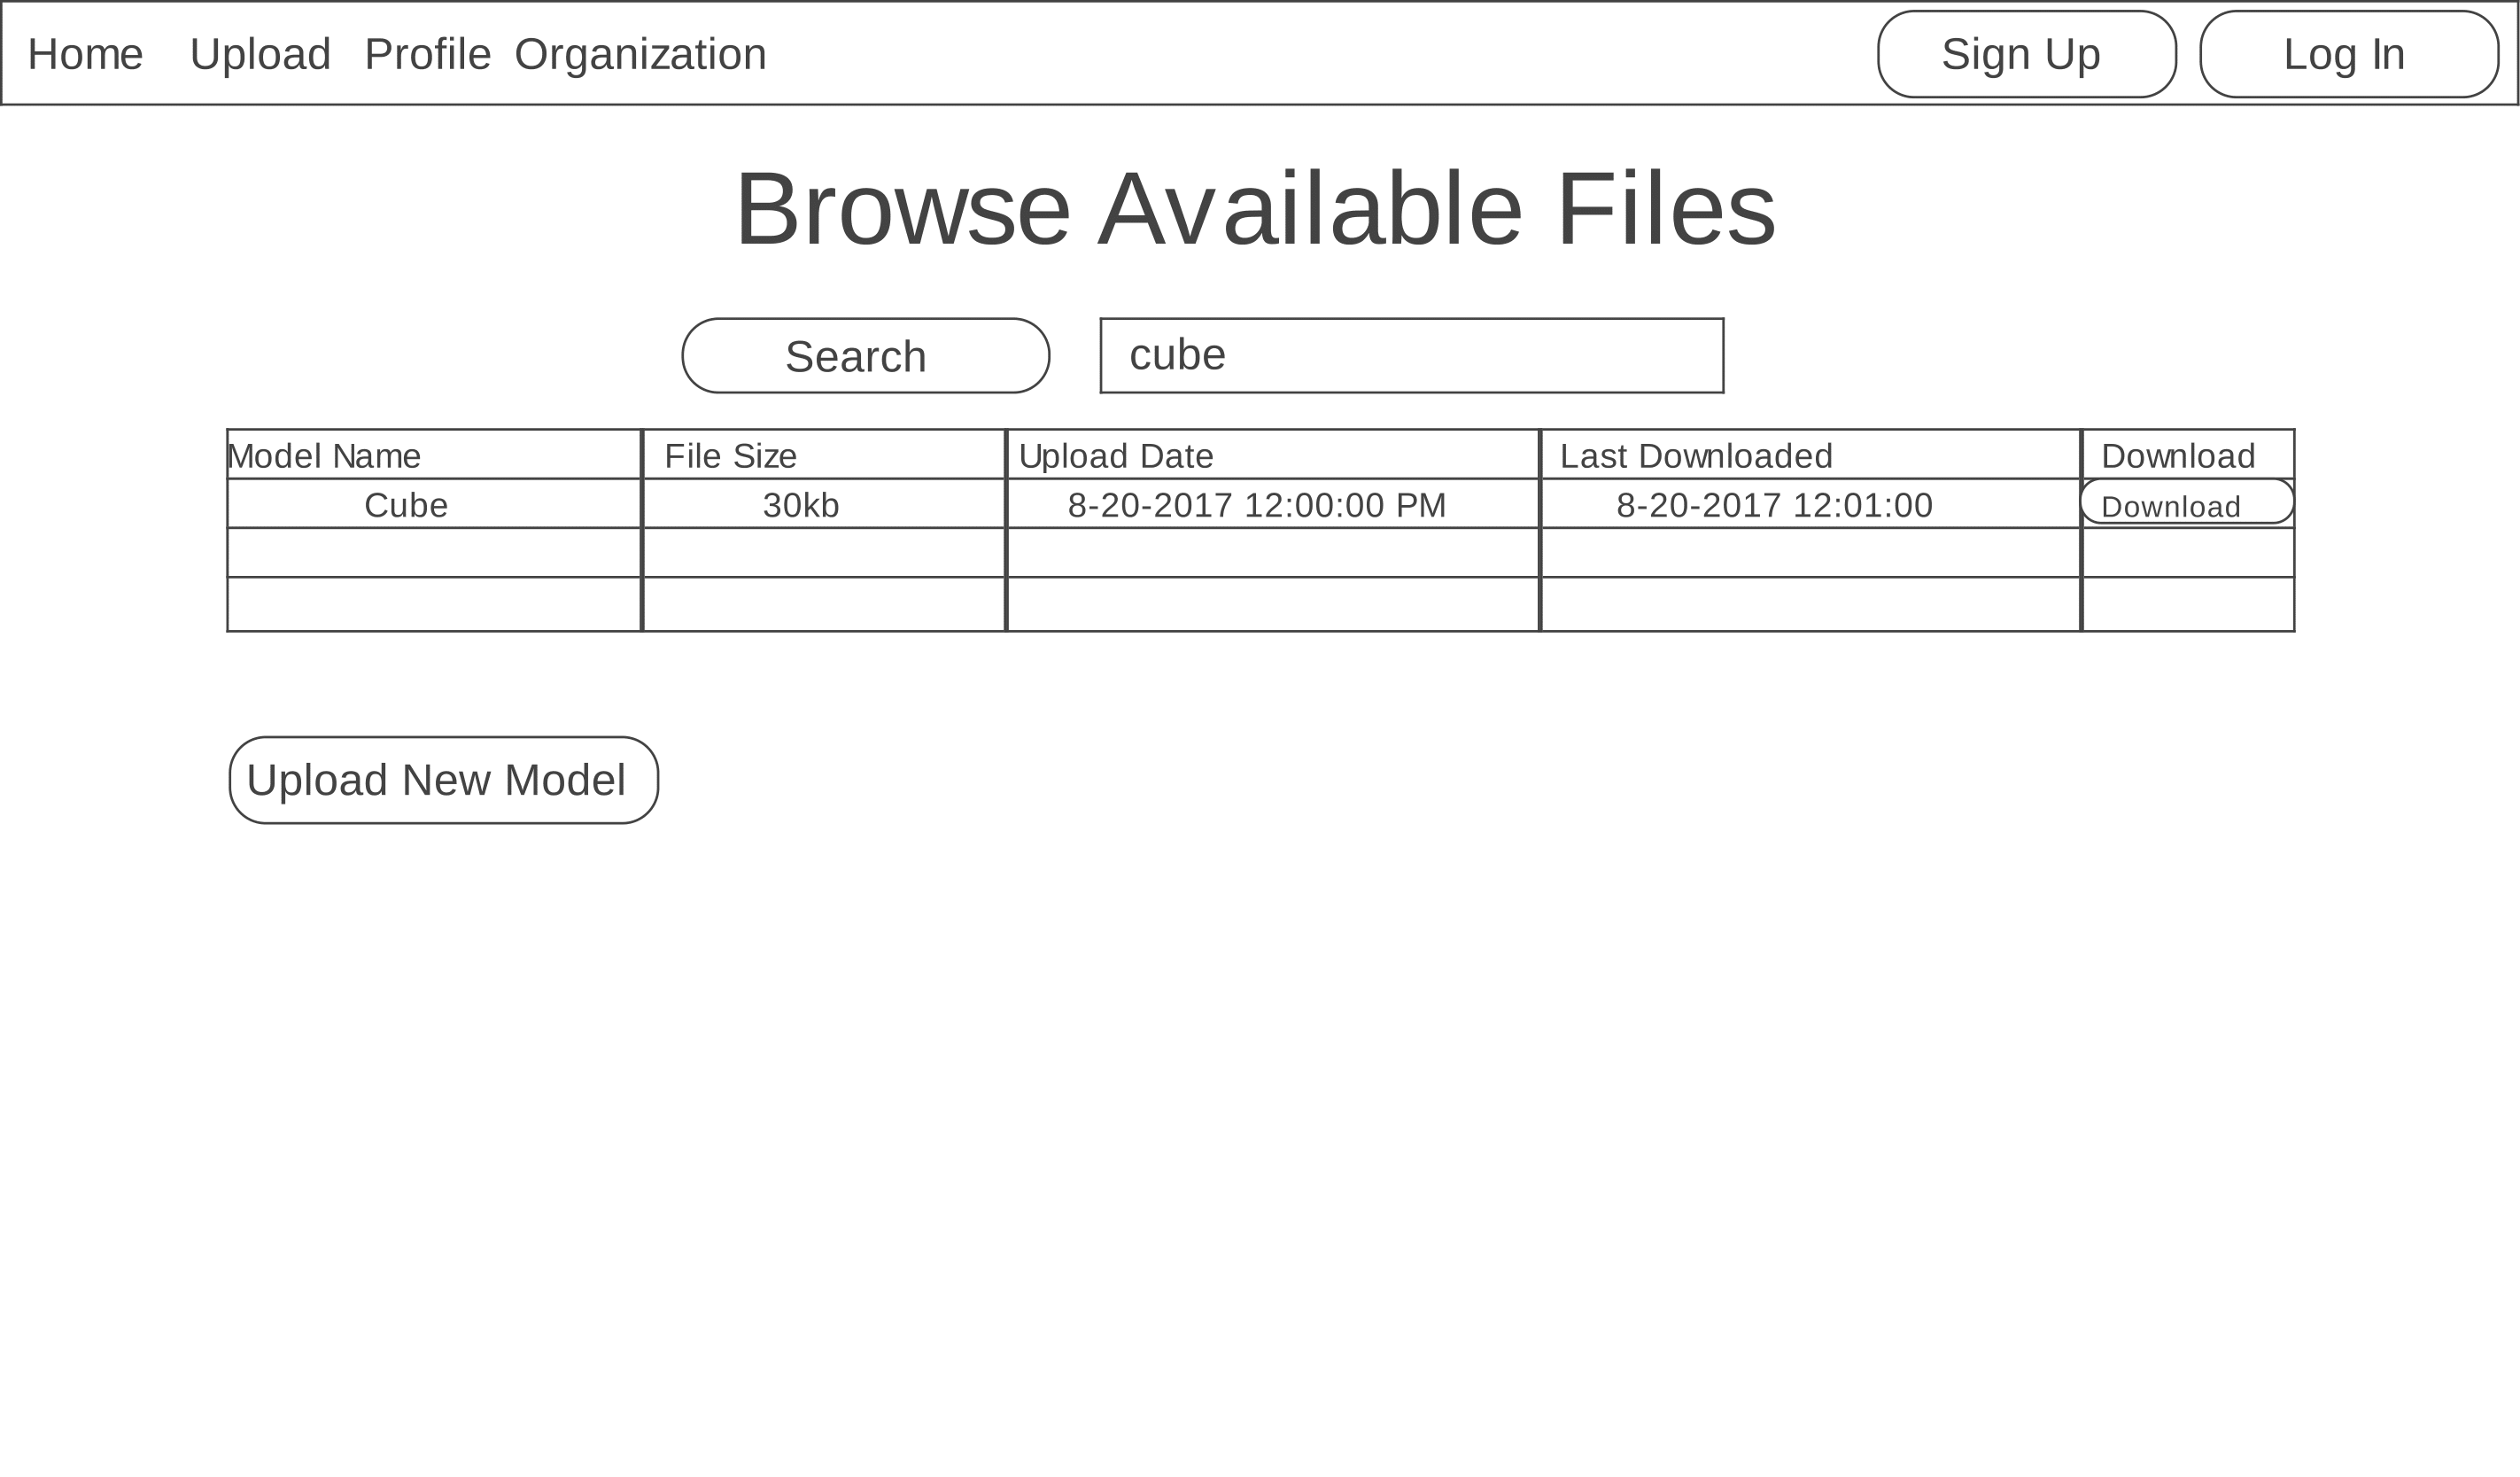
\includegraphics[width=0.6\linewidth]{All}
        \caption{The wireframe for where a user can view all files they have permission to}
    \end{figure}
